% Diese Zeile bitte -nicht- aendern.
\documentclass[course=erap]{aspdoc}
% \documentclass{article}
\usepackage[a4paper, left=3.4cm, right=3cm]{geometry}
\usepackage{graphicx} % Required for inserting images
\usepackage{listings}
\usepackage{booktabs}
\usepackage{amsmath}
\usepackage{blindtext}
\usepackage{float}
% \usepackage[german]{babel}

%%%%%%%%%%%%%%%%%%%%%%%%%%%%%%%%%
%% TODO: Ersetzen Sie in den folgenden Zeilen die entsprechenden -Texte-
%% mit den richtigen Werten.
\newcommand{\theGroup}{223} % Beispiel: 42
\newcommand{\theNumber}{A216} % Beispiel: A123
\author{Pascal Gaertner\and Tushar Khandelwal\and Shaurya Sharma}
\date{Sommersemester 2023}
%%%%%%%%%%%%%%%%%%%%%%%%%%%%%%%%%

% Bitte diese Zeile -nicht- aendern.
\title{Gruppe \theGroup{} -- Abgabe zu Aufgabe \theNumber}

\begin{document}
\maketitle

\section{Einleitung}

\setlength{\parskip}{1em}
\noindent Die Z-Kurve, auch bekannt als Lebesgue-Kurve oder Z-Order-Kurve, ermöglicht die Abbildung mehrdimensionaler Daten in eine eindimensionale Sequenz. Sie findet Anwendung in verschiedenen Bereichen wie Computergrafik, Datenkompression, Datenbanken und Algorithmen für räumliche Indexstrukturen. Die Z-Kurve basiert auf einer linearen Anordnung, die auch als Z-Ordnung oder Morton-Ordnung bezeichnet wird und ermöglicht effiziente Operationen auf mehrdimensionalen Daten, während die Nachbarschaftsbeziehungen erhalten bleiben.
\setlength{\parskip}{1em}

\noindent Der Ansatz der Z-Kurve besteht darin, den Raum rekursiv in Quadranten zu unterteilen und die Punkte innerhalb dieser Unterteilungen in einer spezifischen Reihenfolge zu nummerieren. Diese Reihenfolge gewährleistet, dass benachbarte Punkte im mehrdimensionalen Raum auch in der eindimensionalen Sequenz benachbart sind. Die resultierende Kurve füllt den Raum auf und zeichnet sich durch ihre charakteristische z-förmige Struktur aus, was ihr den Namen Z-Kurve verleiht. In Abbildung 1 ist ein visuelles Beispiel für die Z-Kurve dargestellt, wobei die Grade 1 bis 4 gezeigt werden. Es ist zu erkennen, dass die rekursive Unterteilung der Quadranten mit zunehmendem Grad immer detaillierter wird.
\setlength{\parskip}{1em}

\begin{figure}[H]
        \centering
        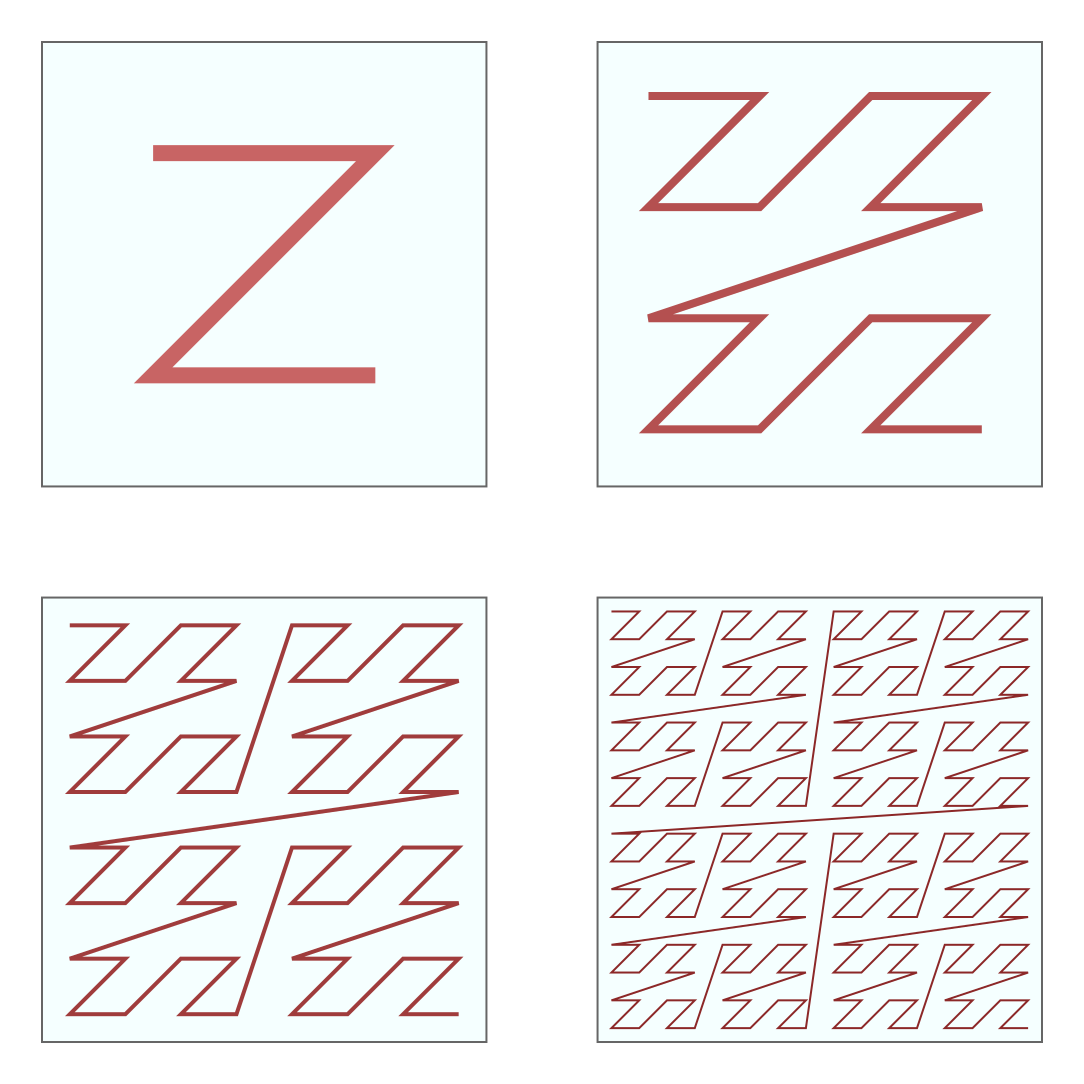
\includegraphics[width=0.4\textwidth, height=6cm]{z_kurve_grad_1_zu_4.png}
        \caption{Grad 1 bis 4 der Z-Kurve}
        \label{fig:Z-Kurve Grad 1 zu 4}
    \end{figure}

\noindent Ein konkretes Beispiel für die Anwendung der Z-Kurve findet sich in der Datenvisualisierung. Hier wird die Z-Kurve verwendet, um mehrdimensionale Daten auf einer eindimensionalen Achse darzustellen. Durch diese Transformation können komplexe Datensätze analysiert werden, indem Trends und Muster in den Daten identifiziert werden. Die Z-Kurve ermöglicht beispielsweise die Visualisierung zeitabhängiger Daten oder multidimensionaler Merkmale auf einer einzigen Achse.
\setlength{\parskip}{1em}

\noindent Ein weiteres Anwendungsbeispiel im Bereich der Datenbanken ist die Verbesserung der Effizienz räumlicher Abfragen mithilfe der Z-Kurve. Durch die Transformation zweidimensionaler Koordinaten in eine eindimensionale Sequenz können geografische Daten effizienter indiziert und durchsucht werden. Dies ermöglicht beispielsweise die schnelle Suche nach nahegelegenen Orten oder das Auffinden von Punkten innerhalb bestimmter geografischer Bereiche.
\setlength{\parskip}{1em}

\noindent Im Rahmen dieses Projekts haben wir uns mit der Implementierung der Z-Kurve in C befasst und drei Funktionen entwickelt. Die erste Funktion berechnet die x- und y-Koordinaten der Z-Kurve bis zu einem gegebenen Grad, der die Anzahl der Iterationen angibt und somit die Feinheit der Raumunterteilung bestimmt. Die berechneten Koordinaten werden in den übergebenen Speicherbereichen gespeichert und als eine SVG-Datei grafisch dargestellt. Die zweite Funktion berechnet die x- und y-Koordinaten für einen gegebenen Z-Wert und speichert sie ebenfalls in den Speicherbereichen. Die letzte Funktion berechnet den Index für eine gegebene Position auf der Kurve und gibt ihn zurück. Alle Funktionen verfügen über Standardparameterwerte, die jedoch vom Nutzer angepasst werden können.
\setlength{\parskip}{1em}

\noindent Diese Ausarbeitung beginnt mit der Beschreibung und Analyse der gewählten 
Lösungs-\\ansätze. Anschließend wird die Korrektheit der Implementierung und des Ansatzes untersucht. Die Performanz der Implementierung wird analysiert und bewertet. Abschließend folgen eine Zusammenfassung der Ergebnisse und ein Ausblick auf zukünftige Entwicklungen des Algorithmus.
\setlength{\parskip}{1em}




\section{Lösungsansatz}
\setlength{\parskip}{1em}
\noindent Im Lösungsansatz wird der Code für die Implementierung der Z-Kurve in C vorgestellt. Zuerst werden einige Entscheidungen erläutert, die für alle drei Funktionen gelten.
\setlength{\parskip}{1em}

\noindent Der Grad wurde auf das Intervall 1 bis 15 beschränkt, da ein Grad größer als 15 die Darstellungsmöglichkeiten eines 32-Bit Integers überschreiten würde. Die Anzahl der Punkte, die von der Gesamtanzahl der Koordinaten abhängt, wird mit einem 32-Bit Integer berechnet. Eine Erweiterung auf einen 64-Bit Integer würde zwar größere Berechnungen ermöglichen, jedoch auch zu einer erheblichen Steigerung der Speicheranforderungen und der Größe des generierten Bildes führen. Da ein Grad von bis zu 15 für die meisten Anwendungsfälle ausreichend ist, wurde die Entscheidung getroffen, bei einem 32-Bit Integer zu bleiben.
\setlength{\parskip}{1em}

\noindent Der Datentyp \texttt{coord\_t} wurde ebenfalls als 32-Bit Integer definiert. Obwohl die größte Koordinate bei einem Grad von 15 nur 15 Bit benötigen würde, haben wir uns dafür entschieden, bei einem 32-Bit Integer zu bleiben. Dies liegt daran, dass bestimmte Implementierungen Shift-Operationen verwenden, bei denen ein 32-Bit Integer von Vorteil ist.
\setlength{\parskip}{1em}

\noindent Nun werden die Lösungsansätze für die erste Funktion besprochen. Diese Funktion hat den Zweck, die x- und y-Koordinaten der Z-Kurve bis zu einem bestimmten Grad zu berechnen und in den übergebenen Arrays x und y abzuspeichern.
\setlength{\parskip}{1em}

\noindent Die rekursive Implementierung besteht aus zwei Funktionen: \texttt{z\_curve\_recursive} und\\ \texttt{z\_curve\_recursive\_helper}. Die Funktion \texttt{z\_curve\_recursive} dient als Einstiegs- \\punkt und nimmt den Grad sowie die Zeiger auf die Arrays \texttt{x} und \texttt{y} entgegen, in denen die berechneten Koordinaten gespeichert werden sollen. Zunächst wird die Gesamtanzahl der Punkte berechnet, die von $4$ hoch den Grad abhängt.
\setlength{\parskip}{1em}

\noindent Die Funktion \texttt{z\_curve\_recursive\_helper} ist rekursiv implementiert und wird von \texttt{z\_curve} aufgerufen. Sie nimmt den Grad, die Startkoordinaten, die Zeiger auf die Arrays \texttt{x} und \texttt{y} sowie den Index entgegen. Die Funktion berechnet die Z-Kurve rekursiv, indem der Raum in Quadranten unterteilt wird. Die Rekursion erfolgt für jeden Quadranten: links oben, rechts oben, links unten und rechts unten. Dabei werden die Startkoordinaten schrittweise verändert, um sich dem gewünschten Punkt anzunähern. Der Grad wird bei jedem rekursiven Aufruf um $1$ verringert. Wenn der Grad den Wert $0$ erreicht hat, werden die berechneten x- und y-Koordinaten basierend auf den Startkoordinaten in den Arrays \texttt{x} und \texttt{y} gespeichert, und der Index wird erhöht. Durch die spezifische Reihenfolge der rekursiven Aufrufe entsteht die Z-Kurve.
\setlength{\parskip}{1em}

\noindent Die Implementierung verwendet die Endrekursion, um die Funktion effizienter zu gestalten und das Risiko eines Stapelüberlaufs bei großen Eingabegrößen zu vermeiden.
\setlength{\parskip}{1em}

\noindent Die Reihenfolge der rekursiven Aufrufe ist wichtig, um die Entstehung der Z-Kurve zu garantieren. Aufgrund dieser Daten-Abhängigkeit ist die rekursive Implementierung nicht für SIMD (Single Instruction, Multiple Data)-Operationen geeignet. Dennoch könnten die letzten vier rekursiven Aufrufe in der Funktion mit SIMD ersetzt werden, da sie unabhängig voneinander sind. Allerdings war die Entwicklung einer SIMD-optimierten Version langsamer als erwartet, und dies aus mehreren Gründen:
\setlength{\parskip}{1em}

\noindent Erstens erfordert SIMD eine zusätzliche Einrichtung und Koordination, um mit den vektorisierten Daten zu arbeiten. Dies beinhaltet das Laden der Daten in SIMD-Register, die korrekte Ausrichtung der Daten und die Behandlung von verbleibenden Iterationen, die nicht in die SIMD-Vektorgröße passen. In unserem Fall ist das Letztere jedoch nicht relevant, da wir immer genau vier Punkte gleichzeitig bearbeiten und die Gesamtanzahl der Punkte ein Vielfaches von vier ist. Bei den nicht-SIMD-Versionen entfällt dieser Einrichtungs- und Koordinierungsaufwand, was zu einem geringeren Overhead und einer besseren Leistung führt.
\setlength{\parskip}{1em}

\noindent Zweitens könnte das schnellere Speicherzugriffsmuster der nicht SIMD-Implementie-\\rung ein Grund sein. Die Standardimplementierung durchläuft und berechnet die Kurve sequenziell, was eine bessere Speicherlokalität und effizientes Caching und Prefetching durch den Prozessor ermöglicht. Bei der SIMD-Implementierung ist dies nicht garantiert. Die Verarbeitung mehrerer Punkte gleichzeitig mit vektorisierten Befehlen führt möglicherweise zu unterschiedlichen Speicherzugriffsmustern, die zu Cache-Fehlern führen und die Berechnung verlangsamen können.

\setlength{\parskip}{1em}

\noindent Der dritte Grund könnte ein menschlicher Fehler sein. SIMD-Implementierungen verwenden im Vergleich zu nicht-SIMD-Versionen komplexere vektorisierte Anweisungen und erfordern spezifische Optimierungen, um die gleichzeitige Verarbeitung mehrerer Punkte zu ermöglichen. Diese erhöhte Komplexität erschwert möglicherweise die Optimierung dieser Implementierung.
\setlength{\parskip}{1em}

\noindent Aufgrund dieser Herausforderungen und der begrenzten Vorteile von SIMD in unserem konkreten Anwendungsfall haben wir uns entschieden, die rekursive Implementierung nicht weiter mit SIMD zu optimieren. Die rekursive nicht-SIMD-Version erzielt bereits gute Leistungsergebnisse und bietet eine bessere Lesbarkeit und Wartbarkeit des Codes.

\noindent Die zweite Implementierung (\texttt{z\_curve\_iterative}) entstand durch die Erkenntnis, dass der Z-Wert durch die bitweise Verzahnung der x- und y-Koordinaten entsteht. \\
Der Prozess der bitweisen Verzahnung besteht darin, beide Koordinaten als Bits zu betrachten und dann von rechts nach links abzuarbeiten, wobei zwischen den x- und y-Bits abgewechselt wird. Bei der Iteration über die Gesamtzahl der Punkte dient der Index als Z-Wert. Da wir den Z-Wert kennen und die x- und y-Koordinaten suchen, müssen wir diesen Prozess umkehren. Dazu arbeiten wir den Index Bit für Bit ab und setzen die entsprechenden x- und y-Bits. Die Anzahl der zu bearbeitenden Bits ergibt sich aus dem Grad der Z-Kurve. Wenn der Grad beispielsweise 5 beträgt, umfasst jede Koordinate 5 Bits. Wenn der Grad 7 beträgt, umfasst jede Koordinate 7 Bits, und so weiter. Die Gesamtanzahl der Bits des Z-Wertes ergibt sich aus der Summe der Bitlängen beider Koordinaten.\\
Um diesen Prozess zu verdeutlichen, betrachten wir Abbildung 2. Hier wird anhand des Z-Wertes 2479 veranschaulicht, wie die x-Koordinate 19 und die y-Koordinate 47 rekonstruiert werden. Die einzelnen Bits des Z-Wertes werden entsprechend den x- und y-Bits zugeordnet, wobei die Reihenfolge und Position der Bits von rechts nach links bestimmt werden. Durch diesen umgekehrten Prozess der bitweisen Verzahnung können die ursprünglichen x- und y-Koordinaten für einen gegebenen Z-Wert ermittelt werden.
\setlength{\parskip}{1em}

\begin{figure}[H]
        \centering
        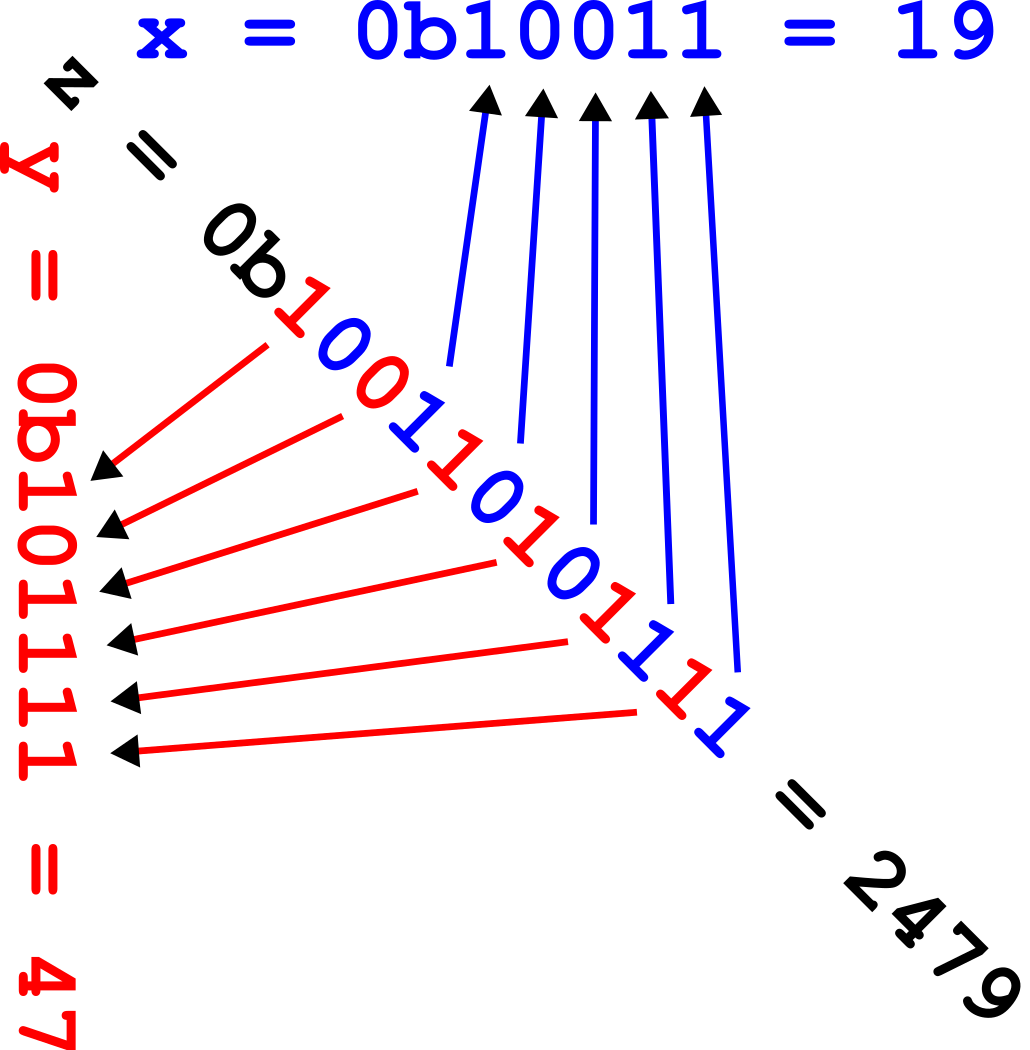
\includegraphics[width=0.4\textwidth, height=6cm]{bit_interleaving.png}
        \caption{Umkehrung der bitweisen Verzahnung}
        \label{fig:Bit Interleaving}
    \end{figure}

\noindent Die zweite Implementierung war immer noch ineffizient, da der Prozess, um die Bitverzahnung umzukehren mit einer for-Schleife durchgeführt wurde. Daher wurde für die dritte Implementierung (\texttt{z\_curve\_magic}) die Idee in Betracht gezogen, diesen Prozess mithilfe von Bit-Shift-Operationen zu optimieren. Dabei stießen wir auf den effizientesten Algorithmus mit Bit-Shifts, der in einem Blog gefunden wurde. Die betreffende Methode wurde mit dem Schlüsselwort "inline" erweitert, um dem Compiler den Hinweis zu geben, den Funktionscode direkt anstatt eines separaten Funktionsaufrufs in den Code einzufügen. Dieses Einbetten des Codes an der Aufrufstelle, auch Inline-Ausführung genannt, kann den Overhead eines Funktionsaufrufs vermeiden und potenziell die Leistung verbessern. Allerdings bleibt die Entscheidung schlussendlich beim Compiler selbst, ob er den Hinweis "inline" beachtet und die Funktion inline ausführt.

\noindent Die Methode \texttt{ReversePart1By1} wurde entwickelt, um den bitweisen Verzahnungsprozess umzukehren und den Wert einer Koordinate zurückzugeben. In dieser Methode wird zuerst eine Maskierung durchgeführt, um die ursprünglichen verzahnten Bits der Koordinate zu isolieren und den Rest auf Null zu setzen. Anschließend werden XOR-Operationen verwendet, um die originalen Bits von "z" mit ihren entsprechend verschobenen Bits zu vergleichen. Dadurch können die verzahnten Bits extrahiert werden, da die Bits, die sich durch die bitweise Verzahnung geändert haben, nach der XOR-Operation den Wert 1 haben. In jeder Iteration wird die Koordinate um eine größere Anzahl von Positionen nach rechts verschoben und eine andere Bitmaske verwendet. Schließlich stellen wir sicher, dass nur die am wenigsten signifikanten 16 Bits beibehalten werden und alle übrigen Bits verworfen werden. Diese Operation ist möglich, ohne Informationen über die Koordinate zu verlieren, da bei einem Grad von 15 die größte Koordinate nur 15 Bits benötigt. Durch die Kombination dieser Schritte wird die bitweise Verzahnung rückgängig gemacht und der ursprüngliche Zustand der Koordinate wiederhergestellt, indem bestimmte Bits isoliert und mit entsprechend verschobenen Bits verglichen werden.

\noindent Für die zweite (\texttt{z\_curve\_iterative}) und dritte (\texttt{z\_curve\_magic}) Implementierung wurden auch SIMD-Varianten entwickelt. Diese Implementierungen haben bestimmte Eigenschaften, die von SIMD-Verarbeitung gut genutzt werden können. Beide Funktionen verwenden Bitmanipulationen, und Bitmanipulationen sind bekanntermaßen gut für SIMD geeignet, da SIMD-Befehle effizient Bitmanipulationen auf mehrere Daten gleichzeitig anwenden können. Darüber hinaus werden bei beiden Implementierungen die Punkte in einer vordefinierten Reihenfolge und unabhängig voneinander berechnet. Diese Art von Datenparallelität lässt sich sehr gut mit SIMD umsetzen. Schließlich weisen beide Implementierungen aufgrund ihrer simplen Schleifenstruktur eine gute SIMD-Kompatibilität auf.

\noindent Die verschiedenen Implementationen der zweiten und dritten Funktion haben sich parallel zur Entwicklung der ersten Funktion entwickelt. Die dritte Methode befasst sich mit der bitweisen Verzahnung, während es bei der zweiten Methode genau wie bei der ersten Methode um die Umkehrung dieser Verzahnung geht. Für beide Methoden wurden Kontrollen eingeführt, um ungültige Z-Werte sowie x- und y-Koordinaten anhand des gegebenen Grades abzufangen und zu behandeln. Dies stellt sicher, dass die Implementierungen robust und fehlerresistent sind und korrekte Ergebnisse liefern.

\noindent In den folgenden Abschnitten werden wir die Genauigkeit und Korrektheit der Implementierung untersuchen und bewerten. Anschließend werden wir die Leistung der Implementierung analysieren und bewerten.
\setlength{\parskip}{1em}

% TODO: Je nach Aufgabenstellung einen der Begriffe wählen
\section{Korrektheit}

\noindent Um die Korrektheit der Z-Kurven-Methoden sicherzustellen, haben wir umfangreiche Tests durchgeführt, indem wir die Ergebnisse jeder Methode mit der rekursiven Methode als Basisfall verglichen haben. Die rekursive Methode ist die direkte Implementierung der Definition der Kurve.

\noindent Wir haben die Z-Kurven-Generierung für Grad von 1 bis 15 getestet. Für jeden Grad haben wir die Koordinaten, die von der rekursiven Methode generiert wurden, mit denen verglichen, die von den anderen Methoden generiert wurden: der iterativen Methode, der Magic-Methode, der iterativen Methode mit SIMD-Optimierung und der Magic-Methode mit SIMD-Optimierung.

\noindent Der Testprozess bestand darin, Z-Kurven-Koordinaten mithilfe der rekursiven Methode zu generieren und sie in den Arrays \texttt{x1} und \texttt{y1} zu speichern. Anschließend haben wir Koordinaten mit jeder der anderen Methoden generiert und sie in den Arrays \texttt{x2}, \texttt{y2}, \texttt{x3}, \texttt{y3}, \texttt{x4}, \texttt{y4}, \texttt{x5} und \texttt{y5} abgelegt.

\noindent Als nächstes haben wir die Koordinaten der rekursiven Methode mit denen jeder anderen Methode, Element für Element, auf mögliche Abweichungen hin verglichen. Dabei haben wir die Indizes festgehalten, an denen die Koordinaten voneinander abweichen, und die Gesamtanzahl der Abweichungen gezählt.

\noindent Durch den Vergleich der Koordinaten, die von der rekursiven Methode mit denen der anderen Methoden generiert wurden, konnten wir die Korrektheit der Implementierung jeder Methode bewerten. Wenn die Koordinaten für alle Methoden identisch waren, haben wir daraus geschlossen, dass die Z-Kurven-Generierung genau und konsistent über die verschiedenen Implementierungen hinweg erfolgte.


\begin{figure}[H]
  \centering
  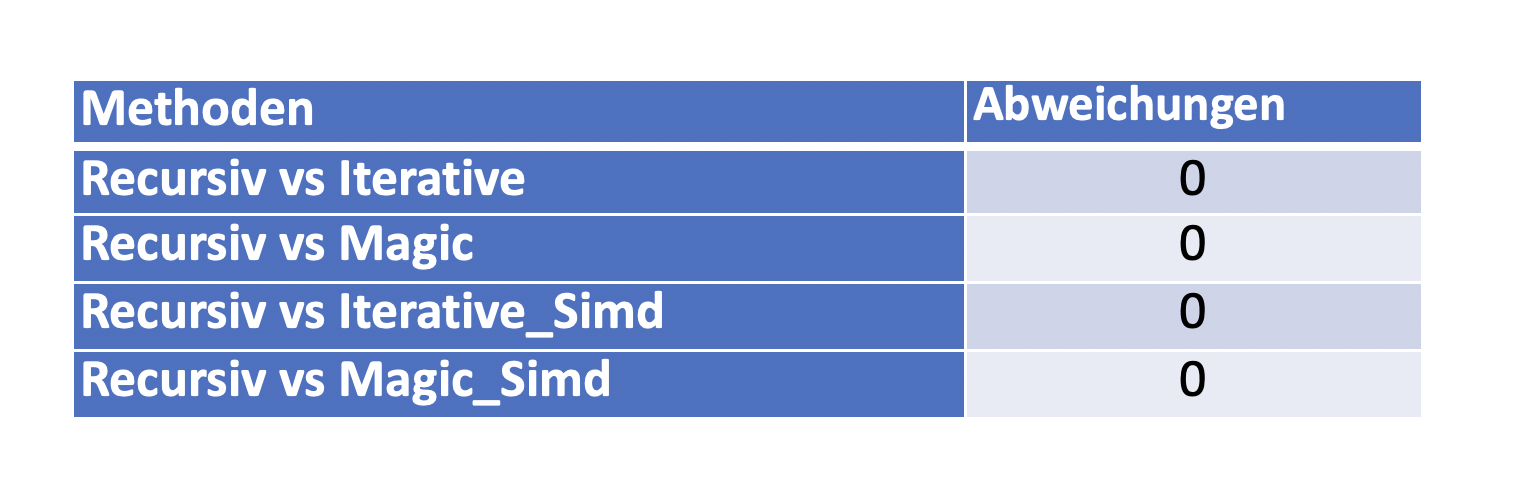
\includegraphics[width=0.9\textwidth]{korrektheit_data.png}
  \caption{Ausgabe von \texttt{testRun\_Method1()}}
  \label{fig:Ausgabe von testRun_Method1()}
\end{figure}

\noindent Um die Analyse zu erleichtern und Abweichungen zu identifizieren, wurden die Testergebnisse auf der Konsole ausgegeben. Die Ausgaben sind in der obigen Tabelle aufgeführt. Die Ausgabe enthielt die Anzahl der gefundenen Abweichungen und die spezifischen Indizes, an denen sich die Koordinaten unterschieden. Dadurch konnte eine einfache Identifizierung und Überprüfung von Inkonsistenzen ermöglicht werden.

\noindent Durch den Vergleich der Z-Kurven-Koordinaten, die von jeder Methode mit der rekursiven Methode als Baseline generiert wurden, konnten wir die Korrektheit der verschiedenen Implementierungen validieren. Dieser umfassende Testansatz lieferte das Vertrauen in die Genauigkeit und Konsistenz der Z-Kurven-Methoden.

\noindent Die Testfunktion \texttt{testRun\_Method1()} wurde verwendet, um die oben genannten Daten zu sammeln und ist in unserem Code enthalten.

\noindent Die Korrektheit der Methoden \texttt{z\_curve\_at()} und \texttt{z\_curve\_pos()} wurde mithilfe der Testmethode \texttt{tester3()} überprüft. In dieser Methode wurden Z-Kurven mit verschiedenen Graden generiert und die erzeugten Koordinaten und Indizes mit den erwarteten Werten verglichen.

\noindent Die Testergebnisse zeigen, dass für alle getesteten Grade von 0 bis 15 keine Abweichungen festgestellt wurden. Weder die Methode \texttt{z\_curve\_at()} noch die Methode \texttt{z\_curve\_pos()} haben fehlerhafte Koordinaten oder Indizes zurückgegeben.

\noindent Somit können wir davon ausgehen, dass die Implementierungen der Methoden\\ \texttt{z\_curve\_at()} und \texttt{z\_curve\_pos()} korrekt sind und die gewünschten Ergebnisse liefern. Die Testmethode \texttt{tester3()} diente dazu, diese Korrektheit zu verifizieren und die Zuverlässigkeit der Methoden sicherzustellen.


\section{Performanzanalyse}

\noindent Für die Leistungsanalyse der Z-Order-Kurve haben wir Experimente mit folgender Hardwarekonfiguration durchgeführt:

Hardware (Rechner Halle):
\begin{itemize}
  \item Architektur: x86\_64
  \item CPU: Intel(R) Xeon(R) CPU E5-2687W v3 @ 3.10GHz
  \item Betriebssystem: Ubuntu 22.04.1 LTS
  \item CFLAGS: -O3 -march=native
\end{itemize}

\noindent Wir haben die Leistung der Z-Order Curve-Implementierung unter Verwendung der gegebenen Hardwarekonfiguration bewertet. Die Implementierung wurde für eine Reihe von Eingabegraden ausgeführt. Zu den gemessenen Leistungsmetriken gehören Laufzeit und Speicherbedarf.

\noindent Die Laufzeitanalyse wurde durch Messung der Ausführungszeit verschiedener Z-Order\\ Curve-Algorithmen/Methoden für verschiedene Eingabegrade durchgeführt. Jede Methode wurde 20 Mal ausgeführt, und die durchschnittliche Laufzeit für jeden Grad bis zu Grad 15 wurde berechnet, um die statistische Zuverlässigkeit zu gewährleisten. Die Laufzeitmessungen wurden unter Verwendung geeigneter Zeitmessungsmechanismen durchgeführt, die von der für die Implementierung verwendeten Programmiersprache oder dem Framework bereitgestellt wurden.

\noindent Wir verglichen verschiedene Implementierungen oder Optimierungsansätze des Z-Order Curve Algorithmus und analysierten ihre Auswirkungen auf die Leistung. Diese Analyse umfasste die Bewertung der Laufzeit jeder Implementierung für verschiedene Eingabegrade.

\noindent Um einen klaren Vergleich zu ermöglichen, präsentieren wir in Abbildung 4 ein umfassendes Diagramm, das die Beziehung zwischen Zeit in Sekunden (y-Achse) und Grad (x-Achse) für fünf verschiedene Implementierungen darstellt.

\begin{figure}[H]
  \centering
  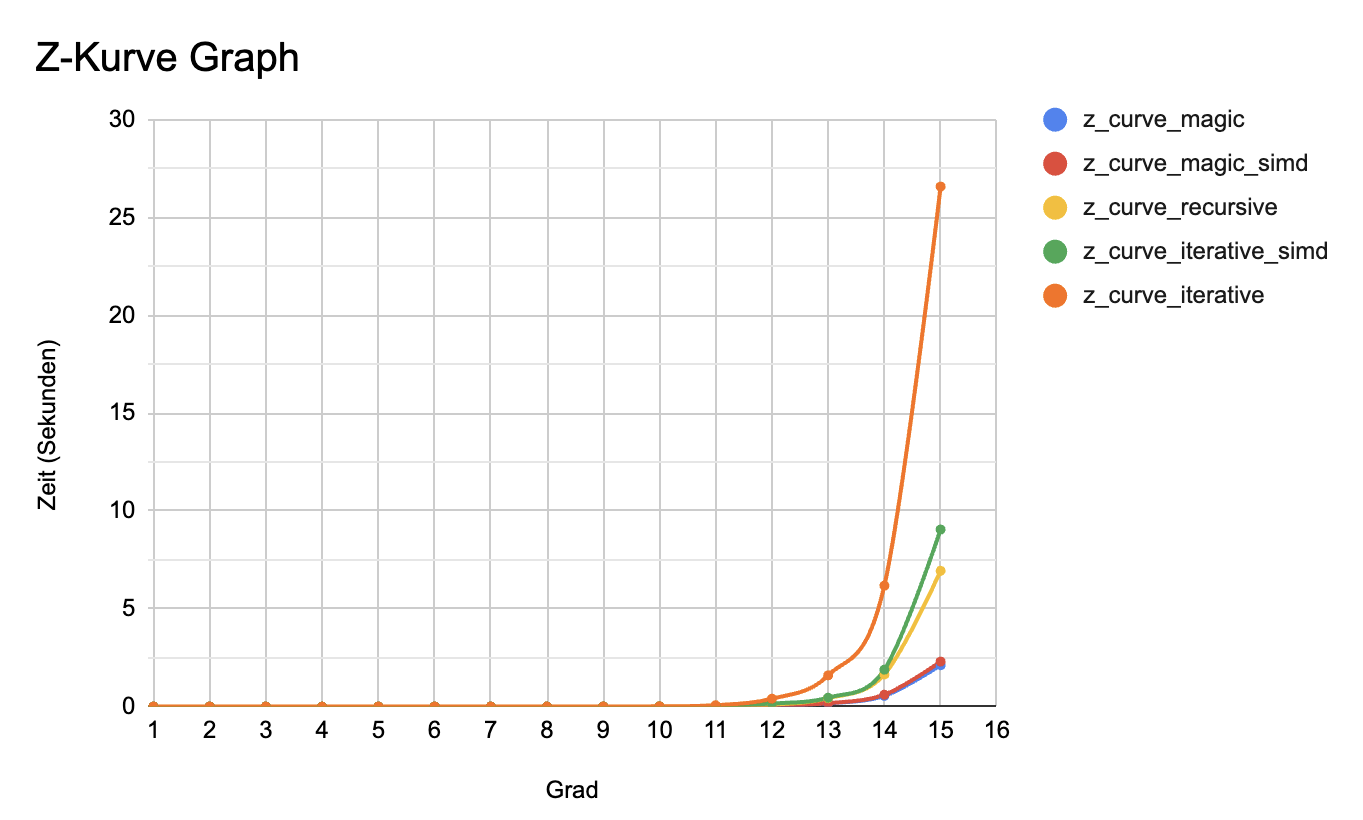
\includegraphics[width=1\textwidth]{z_kurve.png}
  \caption{Beziehung zwischen Zeit und Grad: Vergleich der Implementierungen}
  \label{fig:z kurve graph}
\end{figure}

\noindent Um die Methoden weiter zu vergleichen, berechneten wir die durchschnittliche Laufzeit für jede Methode und fassten die Ergebnisse in Tabelle 1 zusammen.


\noindent Wir haben auch die Zeitkomplexität des von uns implementierten Z-Order Kurven Algorithmus berechnet. Die Ergebnisse zeigen, dass der schnellste Algorithmus/die schnellste Methode, \texttt{z\_curve\_magic()}, eine Zeitkomplexität von $O(4^n)$ hat, wobei n der Eingabegrad ist. Diese Beobachtung bedeutet, dass die Laufzeit des Algorithmus exponentiell mit dem Eingabegrad wächst.



\begin{table}
  \centering
  \scriptsize
  \caption{Grad/Methoden}
\begin{tabular}
    {@{}p{0.7cm}p{1.9cm}p{2.6cm}p{2.2cm}p{2.9cm}p{2.1cm}@{}}
    \toprule
    Grad & z\_curve\_magic & z\_curve\_magic\_simd & z\_curve\_recursive & z\_curve\_iterative\_simd & z\_curve\_iterative \\
    \midrule
    15    & 2.117606545 & 2.299196053 & 6.942717743 & 9.050640106 & 26.57910156 \\
    14    & 0.5462408543 & 0.6086062431 & 1.644544411 & 1.887669945 & 6.183926392 \\
    13    & 0.1641770601 & 0.171334815 & 0.4272080898 & 0.457726717 & 1.596807003 \\
    12    & 0.0297612101 & 0.0402954936 & 0.0969730079 & 0.1577587008 & 0.4033886909 \\
    11    & 0.0087735534 & 0.0096032932 & 0.0198766738 & 0.0341580451 & 0.0691505075 \\
    10    & 0.0032766826 & 0.0022993851 & 0.0067203969 & 0.004974765 & 0.0136007667 \\
    9     & 0.0004712905 & 0.0005461953 & 0.0018441027 & 0.0014517584 & 0.0028929176 \\
    8     & 0.0001384496 & 0.0001394916 & 0.0003829313 & 0.0003207068 & 0.0006730684 \\
    7     & 0.0000266107 & 0.0000333648 & 0.0000935065 & 0.0000798785 & 0.0001515576 \\
    6     & 0.0000060487 & 0.0000081041 & 0.0000247462 & 0.0000173495 & 0.0000402729 \\
    5     & 0.0000011054 & 0.000001945 & 0.0000054274 & 0.0000036603 & 0.0000093163 \\
    4     & 0.0000003096 & 0.0000005171 & 0.0000011488 & 0.000000852 & 0.0000020118 \\
    3     & 0.0000001235 & 0.0000001623 & 0.0000003628 & 0.0000001763 & 0.0000004255 \\
    2     & 0.0000000682 & 0.0000000717 & 0.0000001258 & 0.0000000817 & 0.000000074 \\
    1     & 0.0000000915 & 0.0000000452 & 0.0000000427 & 0.000000046 & 0.0000000306 \\
    \bottomrule
    \end{tabular}
\end{table}
% \bigskip\bigskip\bigskip\bigskip
\noindent Darüber hinaus konnten wir eine erhebliche Leistungssteigerung durch die Verwendung von Cflags feststellen. So betrug beispielsweise die durchschnittliche Laufzeit der Methode \texttt{z\_curve\_magic()} ohne Verwendung von Cflags 28,493687 Sekunden. Nach Anwendung der -O3-Optimierung konnten wir jedoch eine bemerkenswerte Leistungssteigerung beobachten, die zu einer durchschnittlichen Laufzeit von 2,760651 Sekunden führte. Weitere Verbesserungen wurden durch die Einbeziehung von -march=native erzielt, die mit 2,117606 Sekunden die beste durchschnittliche Laufzeit aller Methoden ergab.

\noindent Darüber hinaus untersuchten wir den Speicherbedarf des Z-Order Kurve Algorithmus für jede Implementierung. Unsere Speicheranalyse konzentrierte sich auf die gesamten Speicherzuweisungen für die Punkte während der Ausführung. Die zur Berechnung dieser Zuweisungen verwendete Formel berücksichtigt den Grad (x) des Algorithmus.
\[
\frac{{4^x \times 32 \times 2}}{{8 \times 1024 \times 1024 \times 1024}}
\quad x > 0
\]
% \begin{figure}[H]
%   \centering
%   \includegraphics[width=0.5\textwidth]{formula}
  
%   \label{fig:formula}
% \end{figure}


\noindent Die Grafik in Abbildung 5 zeigt die Speicherzuweisung in Gigabyte (GB) und verdeutlicht ihren exponentiellen Charakter. Die x-Achse stellt den Grad dar, während die y-Achse den Speicher in GB angibt. Bemerkenswert ist, dass bei einem Grad von 15 die Speicherzuteilung 8 GB erreicht, bei einem Grad von 20 jedoch dramatisch auf 8 TB ansteigt!
\bigskip
\begin{figure}[H]
  \centering
  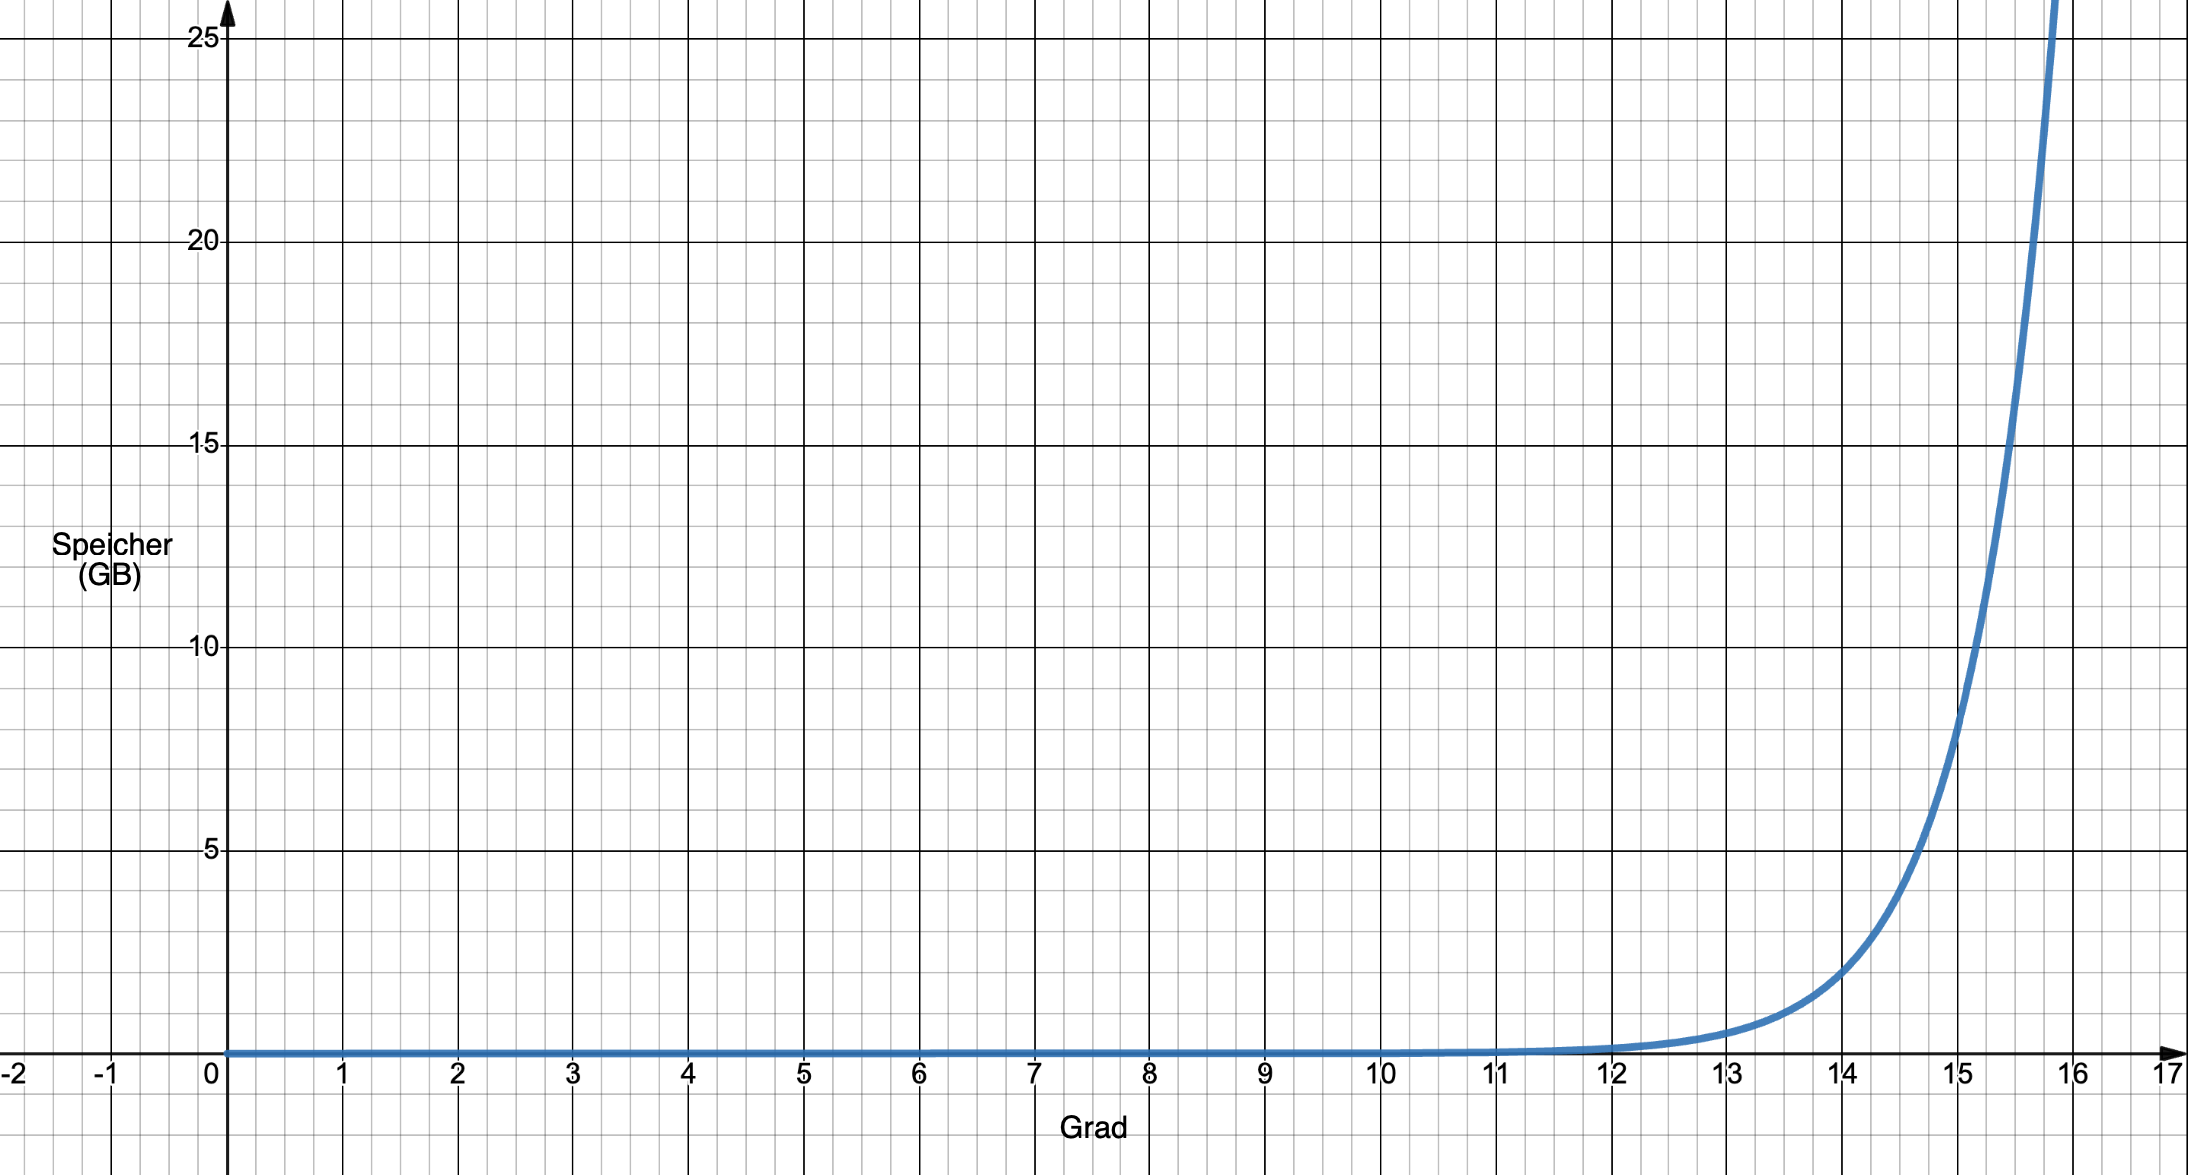
\includegraphics[width=0.9\textwidth]{speicher_graph.png}
  \caption{Speicherzuweisung in Gigabyte (GB) in Abhängigkeit vom Grad}
  \label{fig:speicher Graph}
\end{figure}

\bigskip
\noindent Insgesamt lieferte die Leistungsanalyse des Z-Order Curve Algorithmus auf der gegebenen Hardwarekonfiguration Einblicke in die Effizienz der verschiedenen Implementierungen und deren Auswirkungen auf die Laufzeit. Die Ergebnisse können als wertvolle Orientierungshilfe für die Optimierung der Leistung des Algorithmus und das Verständnis der Implementierungen auf der Grundlage der spezifischen Anforderungen und Einschränkungen der Anwendung dienen.


\section{Zusammenfassung und Ausblick}

\noindent In diesem Projekt haben wir die Implementierung der Z-Kurve in C untersucht und drei Funktionen entwickelt. Die erste Funktion berechnet die Koordinaten bis zu einem bestimmten Grad und wird mittels einer SVG-Datei visualisiert. Die zweite Funktion ermittelt die x- und y-Koordinaten basierend auf einem gegebenen Z-Wert, während die dritte Funktion den Z-Wert anhand von x- und y-Koordinaten berechnet. Wir haben mehrere Implementierungen für diese Funktionen erstellt und miteinander verglichen und analysiert. 

\noindent Ein Ausblick auf zukünftige Entwicklungen des Algorithmus umfasst die Erweiterung der Datentypen auf 64 Bit, um eine Darstellung und Berechnung von Gradstufen über 15 zu ermöglichen. Zudem könnte eine Lookup-Tabelle (LUT) implementiert werden, um die Leistung weiter zu steigern. Darüber hinaus könnten weitere Anwendungen der Z-Kurve erforscht werden beispielsweise im Bereich Datenkompression.

\noindent Insgesamt hat dieses Projekt uns wertvolle Einblicke in die Z-Kurve und ihre Implementierungsmöglichkeiten gegeben. Es hat gezeigt, dass die Z-Kurve in verschiedenen Anwendungsbereichen eine effektive Methode zur Abbildung mehrdimensionaler Daten auf eine eindimensionale Sequenz sein kann und weiteres Potenzial für Verbesserungen und Anwendungen bietet.

% TODO: Fuegen Sie Ihre Quellen der Datei Ausarbeitung.bib hinzu
% Referenzieren Sie diese dann mit \cite{}.
% Beispiel: CR2 ist ein Register der x86-Architektur~\cite{intel2017man}.
\bibliographystyle{plain}
\bibliography{Ausarbeitung}{}

\end{document}